\section{Spark::Sp\-Textured\-Quad\-Sg Class Reference}
\label{classSpark_1_1SpTexturedQuadSg}\index{Spark::SpTexturedQuadSg@{Spark::SpTexturedQuadSg}}
{\tt \#include $<$Sp\-Textured\-Quad\-Sg.h$>$}

Inheritance diagram for Spark::Sp\-Textured\-Quad\-Sg:\begin{figure}[H]
\begin{center}
\leavevmode
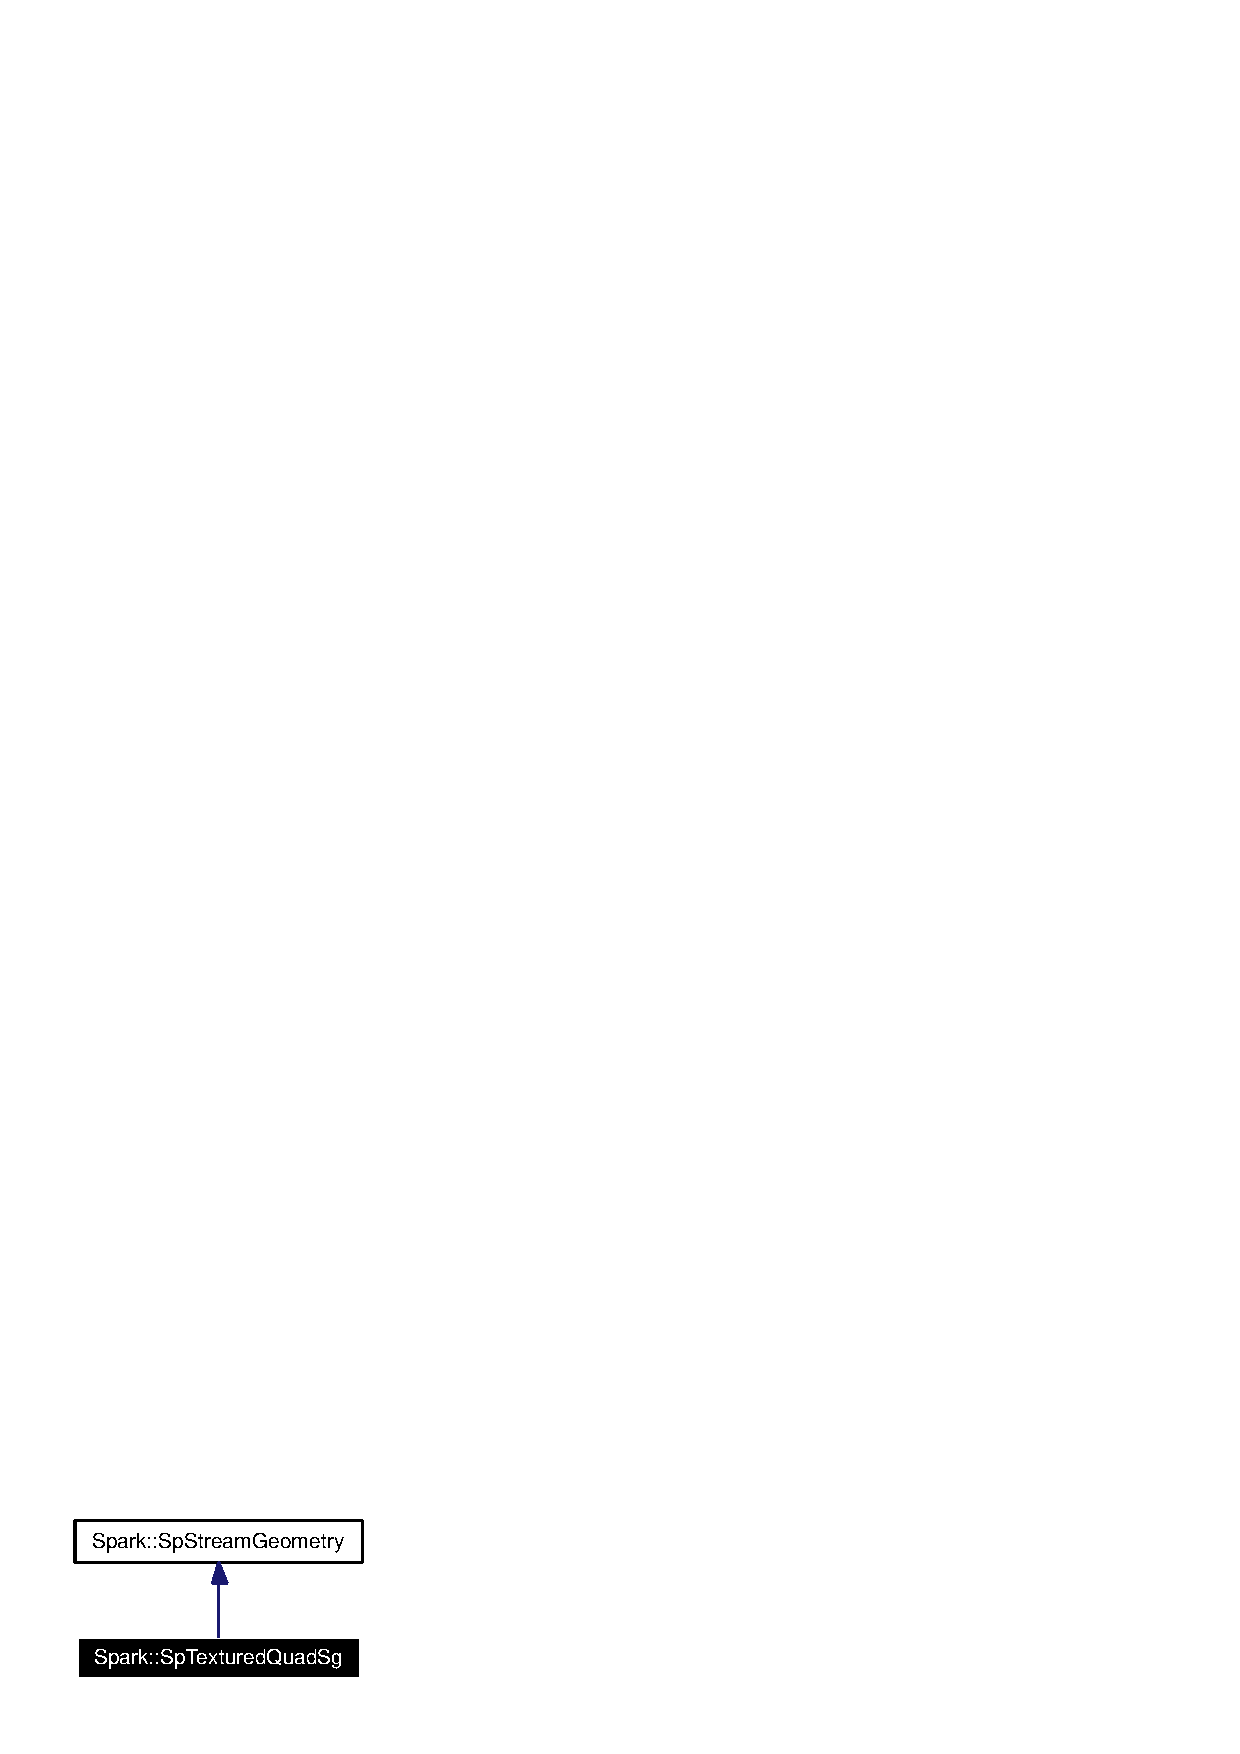
\includegraphics[width=87pt]{classSpark_1_1SpTexturedQuadSg__inherit__graph}
\end{center}
\end{figure}
Collaboration diagram for Spark::Sp\-Textured\-Quad\-Sg:\begin{figure}[H]
\begin{center}
\leavevmode
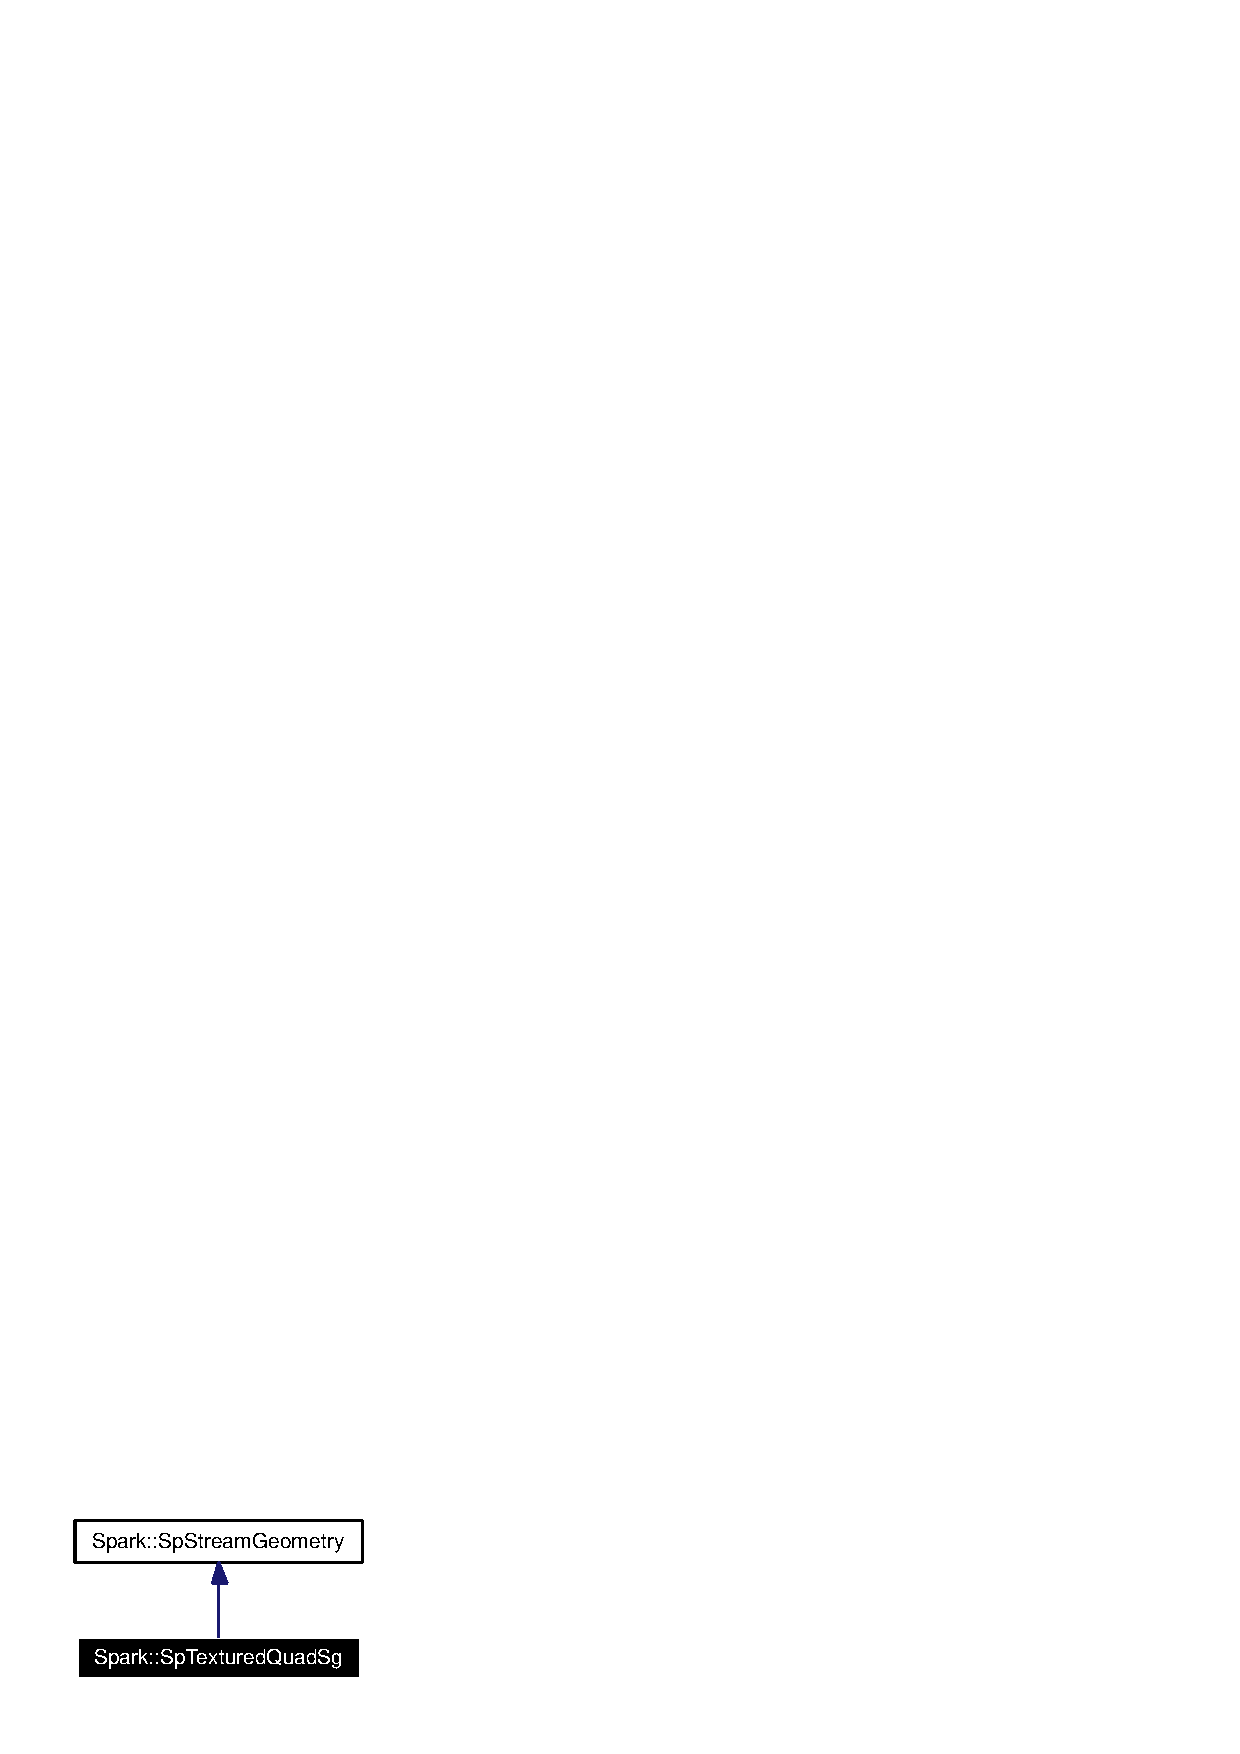
\includegraphics[width=87pt]{classSpark_1_1SpTexturedQuadSg__coll__graph}
\end{center}
\end{figure}


\subsection{Detailed Description}
Quad-based stream geometry w/ texturing support. 

Definition at line 34 of file Sp\-Textured\-Quad\-Sg.h.\subsection*{Public Member Functions}
\begin{CompactItemize}
\item 
{\bf Sp\-Textured\-Quad\-Sg} (float f\-Min\-X=0.0f, float f\-Min\-Y=0.0f, float f\-Max\-X=1.0f, float f\-Max\-Y=1.0f, float f\-Z=0.5f float f\-Min\-S=0.0f, float f\-Min\-T=0.0f, float f\-Max\-S=1.0f, float f\-Max\-T=1.0f))
\begin{CompactList}\small\item\em Construction:. \item\end{CompactList}\item 
virtual {\bf $\sim$Sp\-Textured\-Quad\-Sg} ()
\item 
virtual void {\bf render} ()
\begin{CompactList}\small\item\em Operations:. \item\end{CompactList}\item 
void {\bf set\-Vertex\-Coord\-Rect} (float f\-Min\-X, float f\-Min\-Y, float f\-Max\-X, float f\-Max\-Y, float f\-Z=0.5f)
\item 
void {\bf set\-Tex\-Coord\-Rect} (float f\-Min\-S, float f\-Min\-T, float f\-Max\-S, float f\-Max\-T)
\end{CompactItemize}
\subsection*{Protected Attributes}
\begin{CompactItemize}
\item 
float {\bf m\_\-f\-Min\-X}
\item 
float {\bf m\_\-f\-Min\-Y}
\item 
float {\bf m\_\-f\-Max\-X}
\item 
float {\bf m\_\-f\-Max\-Y}
\item 
float {\bf m\_\-f\-Z}
\item 
float {\bf m\_\-f\-Min\-S}
\item 
float {\bf m\_\-f\-Max\-S}
\item 
float {\bf m\_\-f\-Min\-T}
\item 
float {\bf m\_\-f\-Max\-T}
\end{CompactItemize}


\subsection{Constructor \& Destructor Documentation}
\index{Spark::SpTexturedQuadSg@{Spark::Sp\-Textured\-Quad\-Sg}!SpTexturedQuadSg@{SpTexturedQuadSg}}
\index{SpTexturedQuadSg@{SpTexturedQuadSg}!Spark::SpTexturedQuadSg@{Spark::Sp\-Textured\-Quad\-Sg}}
\subsubsection{\setlength{\rightskip}{0pt plus 5cm}Spark::Sp\-Textured\-Quad\-Sg::Sp\-Textured\-Quad\-Sg (float {\em f\-Min\-X} = {\tt 0.0f}, float {\em f\-Min\-Y} = {\tt 0.0f}, float {\em f\-Max\-X} = {\tt 1.0f}, float {\em f\-Max\-Y} = {\tt 1.0f}, float {\em f\-Z} = {\tt 0.5f\ float\ fMinS\ =\ 0.0f}, float {\em f\-Min\-T} = {\tt 0.0f}, float {\em f\-Max\-S} = {\tt 1.0f}, float {\em f\-Max\-T} = {\tt 1.0f})\hspace{0.3cm}{\tt  [inline]}}\label{classSpark_1_1SpTexturedQuadSg_a0}


Construction:. 

Definition at line 40 of file Sp\-Textured\-Quad\-Sg.h.\index{Spark::SpTexturedQuadSg@{Spark::Sp\-Textured\-Quad\-Sg}!~SpTexturedQuadSg@{$\sim$SpTexturedQuadSg}}
\index{~SpTexturedQuadSg@{$\sim$SpTexturedQuadSg}!Spark::SpTexturedQuadSg@{Spark::Sp\-Textured\-Quad\-Sg}}
\subsubsection{\setlength{\rightskip}{0pt plus 5cm}virtual Spark::Sp\-Textured\-Quad\-Sg::$\sim${\bf Sp\-Textured\-Quad\-Sg} ()\hspace{0.3cm}{\tt  [inline, virtual]}}\label{classSpark_1_1SpTexturedQuadSg_a1}


Definition at line 54 of file Sp\-Textured\-Quad\-Sg.h.

\subsection{Member Function Documentation}
\index{Spark::SpTexturedQuadSg@{Spark::Sp\-Textured\-Quad\-Sg}!render@{render}}
\index{render@{render}!Spark::SpTexturedQuadSg@{Spark::Sp\-Textured\-Quad\-Sg}}
\subsubsection{\setlength{\rightskip}{0pt plus 5cm}virtual void Spark::Sp\-Textured\-Quad\-Sg::render ()\hspace{0.3cm}{\tt  [inline, virtual]}}\label{classSpark_1_1SpTexturedQuadSg_a2}


Operations:. 



Implements {\bf Spark::Sp\-Stream\-Geometry} {\rm (p.\,\pageref{classSpark_1_1SpStreamGeometry_a0})}.

Definition at line 63 of file Sp\-Textured\-Quad\-Sg.h.

References m\_\-f\-Max\-S, m\_\-f\-Max\-T, m\_\-f\-Max\-X, m\_\-f\-Max\-Y, m\_\-f\-Min\-S, m\_\-f\-Min\-T, m\_\-f\-Min\-X, m\_\-f\-Min\-Y, and m\_\-f\-Z.\index{Spark::SpTexturedQuadSg@{Spark::Sp\-Textured\-Quad\-Sg}!setTexCoordRect@{setTexCoordRect}}
\index{setTexCoordRect@{setTexCoordRect}!Spark::SpTexturedQuadSg@{Spark::Sp\-Textured\-Quad\-Sg}}
\subsubsection{\setlength{\rightskip}{0pt plus 5cm}void Spark::Sp\-Textured\-Quad\-Sg::set\-Tex\-Coord\-Rect (float {\em f\-Min\-S}, float {\em f\-Min\-T}, float {\em f\-Max\-S}, float {\em f\-Max\-T})\hspace{0.3cm}{\tt  [inline]}}\label{classSpark_1_1SpTexturedQuadSg_a4}


Definition at line 84 of file Sp\-Textured\-Quad\-Sg.h.

References m\_\-f\-Max\-S, m\_\-f\-Max\-T, m\_\-f\-Min\-S, and m\_\-f\-Min\-T.\index{Spark::SpTexturedQuadSg@{Spark::Sp\-Textured\-Quad\-Sg}!setVertexCoordRect@{setVertexCoordRect}}
\index{setVertexCoordRect@{setVertexCoordRect}!Spark::SpTexturedQuadSg@{Spark::Sp\-Textured\-Quad\-Sg}}
\subsubsection{\setlength{\rightskip}{0pt plus 5cm}void Spark::Sp\-Textured\-Quad\-Sg::set\-Vertex\-Coord\-Rect (float {\em f\-Min\-X}, float {\em f\-Min\-Y}, float {\em f\-Max\-X}, float {\em f\-Max\-Y}, float {\em f\-Z} = {\tt 0.5f})\hspace{0.3cm}{\tt  [inline]}}\label{classSpark_1_1SpTexturedQuadSg_a3}


Definition at line 76 of file Sp\-Textured\-Quad\-Sg.h.

References m\_\-f\-Max\-X, m\_\-f\-Max\-Y, m\_\-f\-Min\-X, m\_\-f\-Min\-Y, and m\_\-f\-Z.

\subsection{Member Data Documentation}
\index{Spark::SpTexturedQuadSg@{Spark::Sp\-Textured\-Quad\-Sg}!m_fMaxS@{m\_\-fMaxS}}
\index{m_fMaxS@{m\_\-fMaxS}!Spark::SpTexturedQuadSg@{Spark::Sp\-Textured\-Quad\-Sg}}
\subsubsection{\setlength{\rightskip}{0pt plus 5cm}float {\bf Spark::Sp\-Textured\-Quad\-Sg::m\_\-f\-Max\-S}\hspace{0.3cm}{\tt  [protected]}}\label{classSpark_1_1SpTexturedQuadSg_p6}


Definition at line 101 of file Sp\-Textured\-Quad\-Sg.h.

Referenced by render(), and set\-Tex\-Coord\-Rect().\index{Spark::SpTexturedQuadSg@{Spark::Sp\-Textured\-Quad\-Sg}!m_fMaxT@{m\_\-fMaxT}}
\index{m_fMaxT@{m\_\-fMaxT}!Spark::SpTexturedQuadSg@{Spark::Sp\-Textured\-Quad\-Sg}}
\subsubsection{\setlength{\rightskip}{0pt plus 5cm}float {\bf Spark::Sp\-Textured\-Quad\-Sg::m\_\-f\-Max\-T}\hspace{0.3cm}{\tt  [protected]}}\label{classSpark_1_1SpTexturedQuadSg_p8}


Definition at line 103 of file Sp\-Textured\-Quad\-Sg.h.

Referenced by render(), and set\-Tex\-Coord\-Rect().\index{Spark::SpTexturedQuadSg@{Spark::Sp\-Textured\-Quad\-Sg}!m_fMaxX@{m\_\-fMaxX}}
\index{m_fMaxX@{m\_\-fMaxX}!Spark::SpTexturedQuadSg@{Spark::Sp\-Textured\-Quad\-Sg}}
\subsubsection{\setlength{\rightskip}{0pt plus 5cm}float {\bf Spark::Sp\-Textured\-Quad\-Sg::m\_\-f\-Max\-X}\hspace{0.3cm}{\tt  [protected]}}\label{classSpark_1_1SpTexturedQuadSg_p2}


Definition at line 95 of file Sp\-Textured\-Quad\-Sg.h.

Referenced by render(), and set\-Vertex\-Coord\-Rect().\index{Spark::SpTexturedQuadSg@{Spark::Sp\-Textured\-Quad\-Sg}!m_fMaxY@{m\_\-fMaxY}}
\index{m_fMaxY@{m\_\-fMaxY}!Spark::SpTexturedQuadSg@{Spark::Sp\-Textured\-Quad\-Sg}}
\subsubsection{\setlength{\rightskip}{0pt plus 5cm}float {\bf Spark::Sp\-Textured\-Quad\-Sg::m\_\-f\-Max\-Y}\hspace{0.3cm}{\tt  [protected]}}\label{classSpark_1_1SpTexturedQuadSg_p3}


Definition at line 96 of file Sp\-Textured\-Quad\-Sg.h.

Referenced by render(), and set\-Vertex\-Coord\-Rect().\index{Spark::SpTexturedQuadSg@{Spark::Sp\-Textured\-Quad\-Sg}!m_fMinS@{m\_\-fMinS}}
\index{m_fMinS@{m\_\-fMinS}!Spark::SpTexturedQuadSg@{Spark::Sp\-Textured\-Quad\-Sg}}
\subsubsection{\setlength{\rightskip}{0pt plus 5cm}float {\bf Spark::Sp\-Textured\-Quad\-Sg::m\_\-f\-Min\-S}\hspace{0.3cm}{\tt  [protected]}}\label{classSpark_1_1SpTexturedQuadSg_p5}


Definition at line 100 of file Sp\-Textured\-Quad\-Sg.h.

Referenced by render(), and set\-Tex\-Coord\-Rect().\index{Spark::SpTexturedQuadSg@{Spark::Sp\-Textured\-Quad\-Sg}!m_fMinT@{m\_\-fMinT}}
\index{m_fMinT@{m\_\-fMinT}!Spark::SpTexturedQuadSg@{Spark::Sp\-Textured\-Quad\-Sg}}
\subsubsection{\setlength{\rightskip}{0pt plus 5cm}float {\bf Spark::Sp\-Textured\-Quad\-Sg::m\_\-f\-Min\-T}\hspace{0.3cm}{\tt  [protected]}}\label{classSpark_1_1SpTexturedQuadSg_p7}


Definition at line 102 of file Sp\-Textured\-Quad\-Sg.h.

Referenced by render(), and set\-Tex\-Coord\-Rect().\index{Spark::SpTexturedQuadSg@{Spark::Sp\-Textured\-Quad\-Sg}!m_fMinX@{m\_\-fMinX}}
\index{m_fMinX@{m\_\-fMinX}!Spark::SpTexturedQuadSg@{Spark::Sp\-Textured\-Quad\-Sg}}
\subsubsection{\setlength{\rightskip}{0pt plus 5cm}float {\bf Spark::Sp\-Textured\-Quad\-Sg::m\_\-f\-Min\-X}\hspace{0.3cm}{\tt  [protected]}}\label{classSpark_1_1SpTexturedQuadSg_p0}


Definition at line 93 of file Sp\-Textured\-Quad\-Sg.h.

Referenced by render(), and set\-Vertex\-Coord\-Rect().\index{Spark::SpTexturedQuadSg@{Spark::Sp\-Textured\-Quad\-Sg}!m_fMinY@{m\_\-fMinY}}
\index{m_fMinY@{m\_\-fMinY}!Spark::SpTexturedQuadSg@{Spark::Sp\-Textured\-Quad\-Sg}}
\subsubsection{\setlength{\rightskip}{0pt plus 5cm}float {\bf Spark::Sp\-Textured\-Quad\-Sg::m\_\-f\-Min\-Y}\hspace{0.3cm}{\tt  [protected]}}\label{classSpark_1_1SpTexturedQuadSg_p1}


Definition at line 94 of file Sp\-Textured\-Quad\-Sg.h.

Referenced by render(), and set\-Vertex\-Coord\-Rect().\index{Spark::SpTexturedQuadSg@{Spark::Sp\-Textured\-Quad\-Sg}!m_fZ@{m\_\-fZ}}
\index{m_fZ@{m\_\-fZ}!Spark::SpTexturedQuadSg@{Spark::Sp\-Textured\-Quad\-Sg}}
\subsubsection{\setlength{\rightskip}{0pt plus 5cm}float {\bf Spark::Sp\-Textured\-Quad\-Sg::m\_\-f\-Z}\hspace{0.3cm}{\tt  [protected]}}\label{classSpark_1_1SpTexturedQuadSg_p4}


Definition at line 98 of file Sp\-Textured\-Quad\-Sg.h.

Referenced by render(), and set\-Vertex\-Coord\-Rect().

The documentation for this class was generated from the following file:\begin{CompactItemize}
\item 
{\bf Sp\-Textured\-Quad\-Sg.h}\end{CompactItemize}
